\documentclass [a4paper] {article}
\usepackage[utf8]{inputenc}
\title{Ciencia de datos, práctica 5}
\author{Juan Casado Ballesteros, Samuel García Gonzalez, Iván Anaya Martín}
\usepackage{Sweave}
\begin{document}
\maketitle

\begin{abstract}
Pendiente
\end{abstract}

\newpage

\newpage
\section{K-vecinos sobre la muestra proporcionada para obtener outliers}
Aplicaremos el algoritmo k-vecinos sobre la muestra que tenemos.
Este algoritmo identificará de forma supervisada en la muestra datos anómalos, para poder obtener los outliers.
En primer lugar deberemos cargar esta desde un archivo .txt.
\begin{Schunk}
\begin{Sinput}
> datos1 <- read.table("datos1.txt")
> datos1
\end{Sinput}
\begin{Soutput}
  Teoria Laboratorio
1      4           4
2      4           3
3      5           5
4      1           1
5      5           4
\end{Soutput}
\end{Schunk}

En segundo lugar calculamos las distancias euclídeas entre todos los puntos
\begin{Schunk}
\begin{Sinput}
> distancias <- as.matrix(dist(datos1))
> distancias
\end{Sinput}
\begin{Soutput}
         1        2        3        4        5
1 0.000000 1.000000 1.414214 4.242641 1.000000
2 1.000000 0.000000 2.236068 3.605551 1.414214
3 1.414214 2.236068 0.000000 5.656854 1.000000
4 4.242641 3.605551 5.656854 0.000000 5.000000
5 1.000000 1.414214 1.000000 5.000000 0.000000
\end{Soutput}
\end{Schunk}

Posteriormente, ordenamos las distancias de cada punto a todos los demás.
\begin{Schunk}
\begin{Sinput}
> for(i in 1:5){
+   distancias[,i] <- sort(distancias[,i])
+ }
> distanciasordenadas <- distancias
\end{Sinput}
\end{Schunk}

Como último paso, reordenamos la matriz para organizarla en función de la distancia
de cada punto a su vecino número 1,2,3...etc. Tras haber organizado la matriz, buscamos en el tercer
vecino, que es el valor k que hemos usado en nuestro análisis para poder identificar los outliers.
\begin{Schunk}
\begin{Sinput}
> outliers_kmeans = list()
> for(i in 1:5){
+   if(distanciasordenadas[4,i]>2.5){
+     outliers_kmeans[[length(outliers_kmeans)+1]] <- datos1[i,]
+   }
+ }
> outliers_kmeans
\end{Sinput}
\begin{Soutput}
[[1]]
  Teoria Laboratorio
4      1           1
\end{Soutput}
\end{Schunk}



\section{Deteccion de datos anómalos sobre la resistencia }

\begin{Schunk}
\begin{Sinput}
> datos2 <- read.table("datos2.txt")
> datos2 <- data.frame(datos2)
> datos2
\end{Sinput}
\begin{Soutput}
  Resistencia Densidad
1         3.0      2.0
2         3.5     12.0
3         4.7      4.1
4         5.2      4.9
5         7.1      6.1
6         6.2      5.2
7        14.0      5.3
\end{Soutput}
\end{Schunk}

\begin{center}
\begin{Schunk}
\begin{Sinput}
> boxplot(datos2$Resistencia, range=1.5, border ="red",horizontal = TRUE)
\end{Sinput}
\end{Schunk}
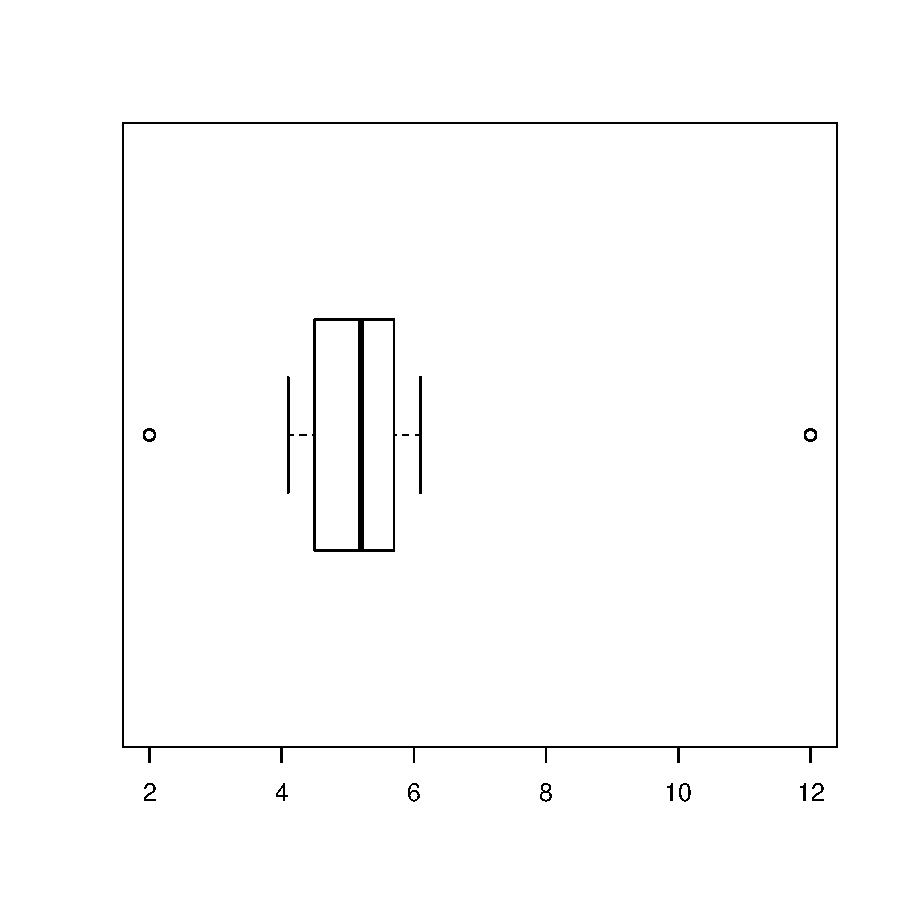
\includegraphics{entrega-plot_caja_bigotes}
\end{center}

\begin{center}
\begin{Schunk}
\begin{Sinput}
> boxplot(datos2$Densidad, range=1.5, border ="red",horizontal = TRUE)
\end{Sinput}
\end{Schunk}
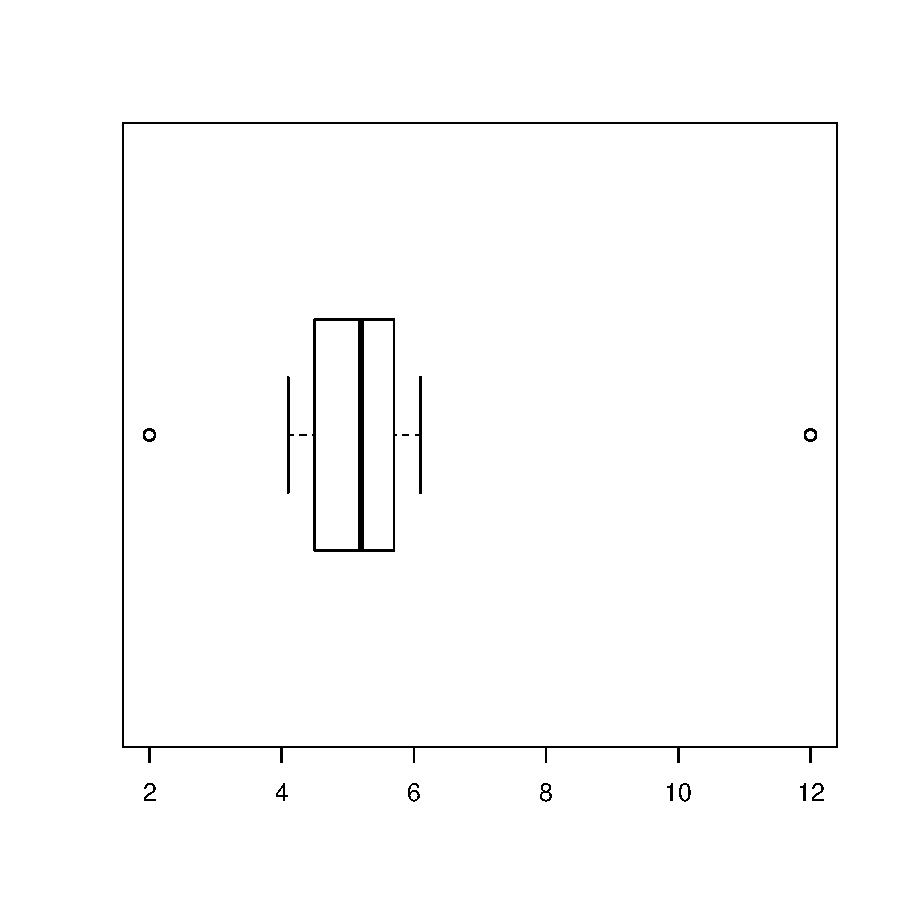
\includegraphics{entrega-plot_caja_bigotes}
\end{center}

\newpage
\section{Dispersión sobre la densidad, desviación típica}

\begin{Schunk}
\begin{Sinput}
> datos2 <- read.table("datos2.txt")
\end{Sinput}
\end{Schunk}

\begin{center}
\begin{Schunk}
\begin{Sinput}
> plotFrecuencyData(datos2$Densidad)
\end{Sinput}
\end{Schunk}
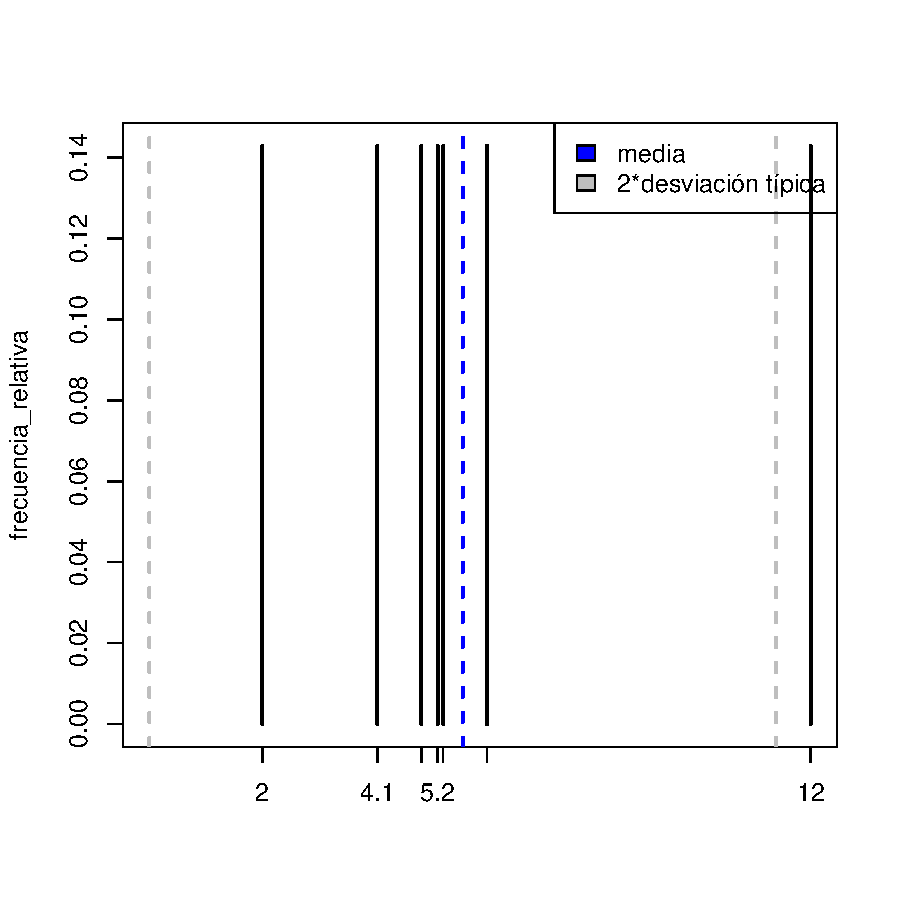
\includegraphics{entrega-desviacion_tipica_densidad}
\end{center}

\begin{center}
\begin{Schunk}
\begin{Sinput}
> plotFrecuencyData(datos2$Resistencia)
\end{Sinput}
\end{Schunk}
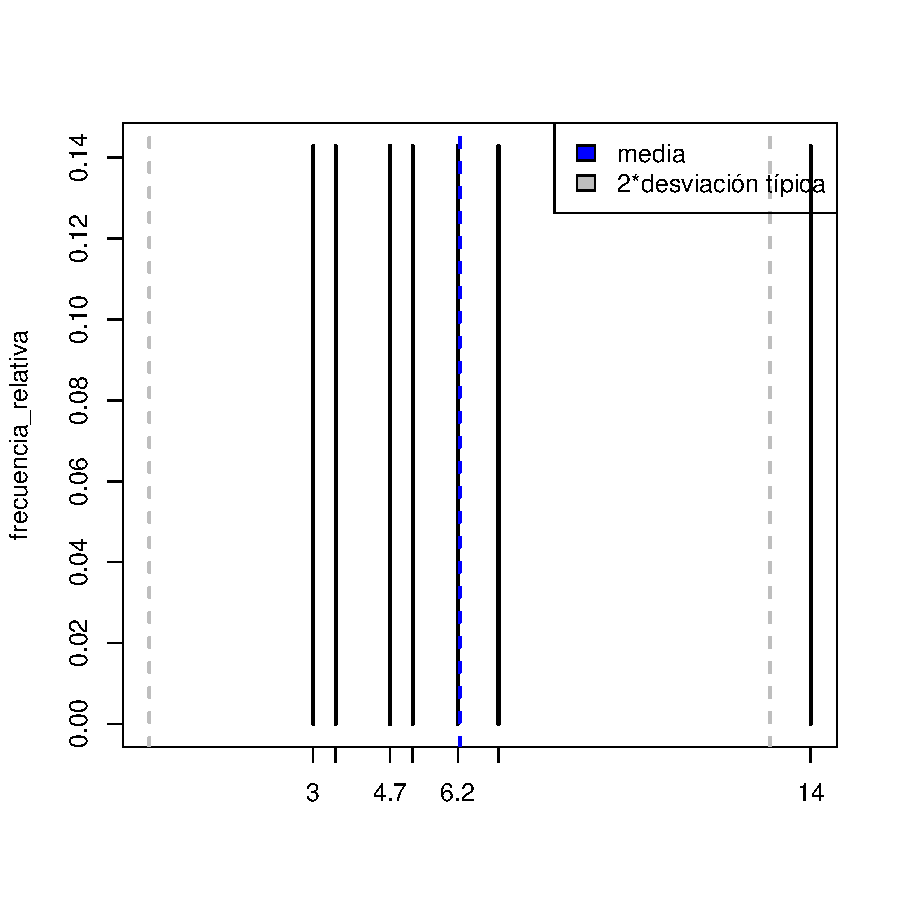
\includegraphics{entrega-desviacion_tipica_resistencia}
\end{center}

\end{document}
